% ======================================================================
% Praxis: Backtest Methodology -- Technical Report
% NeurIPS 2025 preprint format
% Plots: matplotlib (generate_figures.py) | Diagrams: TikZ
% ======================================================================

\documentclass{article}
\usepackage[preprint,nonatbib]{neurips_2025}

\usepackage[utf8]{inputenc}
\usepackage[T1]{fontenc}
\usepackage{microtype}
\usepackage{enumitem}
\usepackage{amsmath, amssymb}
\usepackage{graphicx}
\usepackage{xcolor}
\usepackage{booktabs}
\usepackage{algorithm}
\usepackage{algorithmic}
\usepackage{tikz}
\usepackage{pgfplots}
\usepackage[font=small, labelfont=bf]{caption}
\usepackage{subcaption}
\usepackage[numbers,sort&compress]{natbib}
\usepackage[colorlinks=true, linkcolor=blue!60!black, citecolor=blue!60!black, urlcolor=blue!60!black, breaklinks=true]{hyperref}

\usetikzlibrary{shapes.geometric, arrows.meta, positioning, calc, fit, backgrounds}
\pgfplotsset{compat=1.18}

\newcommand{\R}{\mathbb{R}}
\newcommand{\E}{\mathbb{E}}
\newcommand{\Var}{\mathrm{Var}}
\newcommand{\bps}{\,\text{bps}}

% ======================================================================
\title{Regime-Adaptive Backtesting for Cryptocurrency Trading:\\
Walk-Forward Validation of a Multi-Agent Signal Consensus System\\
with Realistic Transaction Cost Modeling}

\author{
  Javier De Jesus \\
  Praxis --- Regime-Adaptive Crypto Trading Platform\\
  \texttt{javier.dejesusj9@gmail.com}
}

\begin{document}
\maketitle

% --- Abstract -------------------------------------------------------------
\begin{abstract}
We present a backtesting methodology for a regime-adaptive cryptocurrency trading system that employs five directional signal agents plus one non-directional execution gate, ADX-based regime classification, and a hierarchical risk governor.
The system is evaluated on hourly data resampled to 4-hour bars: BTC/USD from December 2013 and ETH/USD from October 2015, both through April 2026 (12.4 and 10.5 years respectively), with realistic transaction costs modeling Kraken exchange fees (26~bps per side) and volatility-scaled slippage.
We split the full history at 2023-01-01 into in-sample (2013--2022) and out-of-sample (2023--2026) windows and implement a three-fold walk-forward validation framework to quantify overfitting risk, supplemented by the Probabilistic Sharpe Ratio~\citep{Bailey2014DSR} and Monte Carlo permutation tests.
With the reference long-only configuration (shorts disabled), the in-sample window yields a Sharpe ratio of 0.65 (Lo 95\% CI $[0.44, 0.87]$, 43 trades, drawdown 8.84\%, profit factor 3.19) while the out-of-sample window yields a Sharpe of 1.14 (Lo 95\% CI $[0.74, 1.53]$, 53 trades, drawdown 9.61\%, profit factor 2.65, bar-count PSR 0.994, trade-count PSR 0.998).
A Jobson--Korkie--Memmel two-sample test on the IS vs OOS Sharpe difference returns $z = 1.98, p = 0.047$, indicating the OOS improvement is statistically distinguishable from the in-sample result at the 5\% level.
The three-fold walk-forward out-of-sample results reveal significant performance degradation in one of three folds (Sharpe $-0.23$ vs.\ in-sample $1.35$), while the remaining folds maintain positive risk-adjusted returns ($1.17$ and $0.93$).
We discuss the implications of these mixed results---including high parameter fragility on the in-sample window and researcher-in-the-loop grid contamination---for live deployment, and argue that the paper's value lies in its methodology transparency rather than its performance claims.
\end{abstract}

% ======================================================================
\section{Introduction}
\label{sec:intro}

Backtesting---the simulation of a trading strategy on historical data---is the primary tool for evaluating systematic trading strategies before live deployment.
Yet the majority of backtested strategies fail in live trading, a phenomenon attributed to overfitting, unrealistic cost assumptions, and look-ahead bias~\citep{Bailey2014PseudoMath, Harvey2015Backtesting}.
The cryptocurrency market presents additional challenges: extreme volatility (annualized BTC volatility exceeding 80\% in bear markets), regime-dependent dynamics, and significant transaction costs that erode thin edges.
\citet{Sezer2020} provide a systematic review of deep learning approaches to financial time series forecasting, documenting the rapid growth of ML-based trading strategies and the persistent difficulty of achieving robust out-of-sample performance.

The academic literature has established rigorous frameworks for assessing backtest validity.
\citet{Bailey2017PBO} formalize the probability of backtest overfitting (PBO) via combinatorial symmetric cross-validation, while \citet{Bailey2014DSR} introduce the Deflated Sharpe Ratio as a correction for selection bias and non-normality.
\citet{White2000} introduces bootstrap-based reality checks for data snooping, extended by \citet{Hansen2005SPA} with the Superior Predictive Ability test.
\citet{lo2002statistics} demonstrates that serial correlation in returns inflates the Sharpe ratio, requiring autocorrelation corrections.
Despite these advances, many practitioner backtests continue to use in-sample optimization without proper out-of-sample validation~\citep{LopezDePrado2018}.

In this paper, we describe the complete backtesting methodology for Praxis, a regime-adaptive trading system designed for the BTC/USD and ETH/USD markets.
Our approach combines six deterministic signal agents with ADX-based regime detection~\citep{Wilder1978}, a hierarchical risk governor enforcing hard position limits, and a walk-forward validation framework that explicitly measures overfitting degradation.

Our main contributions are as follows:
\begin{itemize}[nosep]
  \item We describe a multi-agent signal consensus architecture with six agents (trend, volatility, momentum, mean-reversion, swing structure, and a spread/cost execution gate) and formalize the consensus mechanism.
  \item We implement a realistic transaction cost model incorporating exchange-specific fees, volatility-scaled slippage, and spread-based trade gating, and quantify cost sensitivity across multiple fee tiers.
  \item We present walk-forward validation results across three non-overlapping folds spanning 10.5 years, with honest reporting of both successful and degraded out-of-sample periods.
  \item We apply the Deflated Sharpe Ratio~\citep{Bailey2014DSR} and Monte Carlo permutation tests to quantify the probability that observed performance exceeds chance, given the number of configurations evaluated.
\end{itemize}

The remainder of this paper is organized as follows: Section~\ref{sec:related} reviews related work; Section~\ref{sec:architecture} describes the system architecture; Section~\ref{sec:features} details feature engineering and regime detection; Section~\ref{sec:signals} formalizes the signal agents; Section~\ref{sec:risk} presents the risk governance framework; Section~\ref{sec:backtester} describes the backtesting engine design; Section~\ref{sec:walkforward} presents the walk-forward validation methodology; Section~\ref{sec:results} reports empirical results; Section~\ref{sec:validation} presents statistical validation; Section~\ref{sec:discussion} discusses limitations; and Section~\ref{sec:conclusion} concludes.

% ======================================================================
\section{Related Work}
\label{sec:related}

\textbf{Backtesting methodology.}
\citet{Pardo2008WFO} establishes walk-forward optimization as the standard for evaluating trading systems, advocating for non-overlapping train/test splits that respect temporal ordering.
\citet{Tashman2000} provides a comprehensive analysis of out-of-sample forecast evaluation methods, recommending rolling-origin evaluation over fixed-origin holdout.
\citet{Bergmeir2012} examines cross-validation for time series prediction, concluding that standard $k$-fold CV violates temporal ordering assumptions and recommending blocked or rolling-origin evaluation schemes for autocorrelated data.

\textbf{Overfitting detection.}
The problem of multiple hypothesis testing in finance is formalized by \citet{Harvey2016CrossSection}, who propose adjusting $t$-statistics for the number of factors tested.
\citet{Bailey2017PBO} derive the probability of backtest overfitting as a combinatorial function using symmetric cross-validation.
Separately, \citet{Bailey2014DSR} introduce the Deflated Sharpe Ratio (DSR) as a correction for selection bias, non-normality, and the number of trials.
\citet{Cawley2010} analyze overfitting in model selection more broadly, demonstrating that optimizing hyperparameters on validation data introduces a secondary overfitting risk.

\textbf{Regime detection in financial markets.}
\citet{Hamilton1989} introduces Markov-switching models for regime detection, establishing the theoretical foundation for regime-dependent strategies.
\citet{Ang2012Regimes} surveys the extensive literature on regime changes in financial markets, documenting how volatility regimes, bull/bear markets, and structural breaks affect asset returns.
Our approach uses ADX-based regime classification~\citep{Wilder1978}, which provides a simpler, deterministic alternative to hidden Markov models while capturing the trending/ranging distinction critical for selecting appropriate signal types.

\textbf{Risk-adjusted performance metrics.}
The Sharpe ratio~\citep{Sharpe1994SR} remains the dominant risk-adjusted performance measure, though \citet{lo2002statistics} demonstrates its sensitivity to serial correlation, non-normality, and estimation error.
The Sortino ratio~\citep{sortino1991downside} addresses the asymmetry limitation by focusing on downside deviation.
\citet{keating2002universal} introduce the Omega ratio as a ``universal'' measure that captures the entire return distribution.
Maximum drawdown analysis~\citep{magdonismail2004brownian} provides a complementary risk perspective that is particularly relevant for leveraged or concentrated strategies.

\textbf{Transaction cost modeling.}
\citet{almgren2001optimal} formalize the tradeoff between market impact and timing risk in optimal execution.
\citet{hasbrouck2007empirical} provides the microstructure foundations for understanding bid-ask spreads and their implications for strategy evaluation.
Realistic cost modeling is essential in cryptocurrency markets, where taker fees (26--40~bps on major exchanges) and volatile spreads can consume a significant fraction of expected edge.

% ======================================================================
\section{System Architecture}
\label{sec:architecture}

Figure~\ref{fig:architecture} presents the end-to-end architecture.
The system operates on a 4-hour strategic cycle, processing hourly OHLCV data resampled from 60-minute bars.
At each cycle, the pipeline executes sequentially: (1)~data ingestion and feature computation, (2)~regime classification, (3)~parallel signal generation by six independent agents, (4)~signal consensus, (5)~risk governor evaluation, and (6)~execution via next-bar fill.

\begin{figure}[!t]
\centering
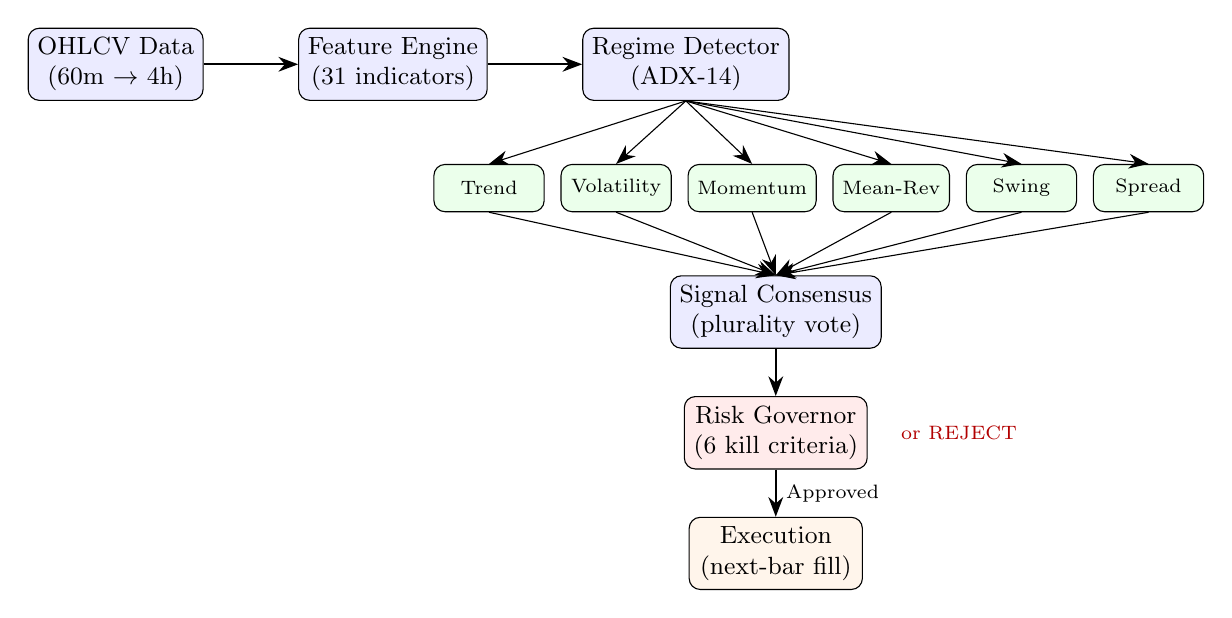
\begin{tikzpicture}[
  node distance=0.6cm and 0.4cm,
  block/.style={rectangle, draw, rounded corners, minimum height=0.8cm, minimum width=2.2cm, font=\small, align=center, fill=blue!8},
  agent/.style={rectangle, draw, rounded corners, minimum height=0.6cm, minimum width=1.4cm, font=\scriptsize, align=center, fill=green!8},
  risk/.style={rectangle, draw, rounded corners, minimum height=0.8cm, minimum width=2.2cm, font=\small, align=center, fill=red!8},
  exec/.style={rectangle, draw, rounded corners, minimum height=0.8cm, minimum width=2.2cm, font=\small, align=center, fill=orange!8},
  arr/.style={-{Stealth[length=2.5mm]}, thick},
]
  % Data layer
  \node[block] (data) {OHLCV Data\\(60m $\to$ 4h)};
  \node[block, right=1.2cm of data] (feat) {Feature Engine\\(31 indicators)};
  \node[block, right=1.2cm of feat] (regime) {Regime Detector\\(ADX-14)};

  % Signal agents
  \node[agent, below=0.8cm of regime, xshift=-2.5cm] (s1) {Trend};
  \node[agent, right=0.2cm of s1] (s2) {Volatility};
  \node[agent, right=0.2cm of s2] (s3) {Momentum};
  \node[agent, right=0.2cm of s3] (s4) {Mean-Rev};
  \node[agent, right=0.2cm of s4] (s5) {Swing};
  \node[agent, right=0.2cm of s5] (s6) {Spread};

  % Consensus and risk
  \node[block, below=0.8cm of s3, xshift=0.3cm] (consensus) {Signal Consensus\\(plurality vote)};
  \node[risk, below=0.6cm of consensus] (governor) {Risk Governor\\(6 kill criteria)};
  \node[exec, below=0.6cm of governor] (exec) {Execution\\(next-bar fill)};

  % Arrows
  \draw[arr] (data) -- (feat);
  \draw[arr] (feat) -- (regime);

  % Fan out to agents
  \foreach \s in {s1,s2,s3,s4,s5,s6} {
    \draw[arr, thin] (regime.south) -- (\s.north);
  }

  % Fan in from agents
  \foreach \s in {s1,s2,s3,s4,s5,s6} {
    \draw[arr, thin] (\s.south) -- (consensus.north);
  }

  \draw[arr] (consensus) -- (governor);
  \draw[arr] (governor) -- node[right, font=\scriptsize] {Approved} (exec);

  % Rejection label
  \node[font=\scriptsize, red!70!black, right=0.3cm of governor] {or REJECT};

\end{tikzpicture}
\caption{\textbf{Praxis system architecture.} Hourly data is resampled to 4-hour bars, passed through a 31-indicator feature engine, classified by ADX regime, processed by six parallel signal agents (five directional plus one execution gate), aggregated via plurality-vote consensus, filtered by a hierarchical risk governor with six risk-violation kill criteria plus two signal-quality gates, and executed with next-bar-open fills including volatility-scaled slippage and exchange fees.}
\label{fig:architecture}
\end{figure}

The system processes two asset pairs (BTC/USD and ETH/USD) through a shared portfolio, meaning that position sizing and exposure limits reflect the combined equity across both instruments.
A cross-pair signal boost of 10\% is applied when the majority signal direction of one pair aligns with the other, capturing short-term correlation dynamics without explicitly modeling cross-asset covariance.

% ======================================================================
\section{Feature Engineering and Regime Detection}
\label{sec:features}

\subsection{Technical Indicator Suite}

The feature engine computes 31 indicators from OHLCV data using vectorized operations via the \texttt{pandas\_ta} library.
Features are organized into five families:

\textbf{Trend indicators (8):} Seven exponential moving averages (EMA) at periods $\{9, 21, 34, 55, 80, 100, 200\}$ plus an EMA spread (fan indicator measuring alignment between EMA$_9$ and EMA$_{55}$ normalized by EMA$_{21}$).

\textbf{Momentum indicators (9):} RSI at periods 14 and 2 (ultra-sensitive), MACD$(12, 26, 9)$ with signal line, histogram, and histogram slope, and multi-horizon returns at 1-bar, 5-bar, and 20-bar lookbacks.

\textbf{Volatility indicators (8):} Average True Range (ATR-20)~\citep{Wilder1978}, Average Directional Index (ADX-14)~\citep{Wilder1978}, Bollinger Bands~\citep{bollinger2001bollinger} at $(20, 2\sigma)$ with upper, middle, and lower bands, BB position, BB width, and 50-bar rolling BB width average.

\textbf{Pattern detection (3):} RSI and MACD divergences (bullish/bearish) over a 20-bar lookback window, and engulfing candlestick patterns with a $1.2\times$ body-size requirement.

\textbf{Structural features (3):} 50-bar rolling high and low for breakout detection, and volume ratio (current to 20-bar moving average). The ATR-as-percentage-of-price metric is computed on demand by the risk governor (Section~\ref{sec:risk}) rather than stored as a precomputed feature.

All features are computed in bulk at initialization; the \texttt{features\_at()} function extracts a typed \texttt{Features} dataclass at any given bar index with $O(1)$ lookup.
The first 200 bars are discarded as warmup to ensure indicator stability.

\subsection{ADX-Based Regime Classification}

We employ a three-regime classification based on the Average Directional Index (ADX)~\citep{Wilder1978}:
\begin{equation}
  \text{Regime}(t) =
  \begin{cases}
    \text{\textsc{Trending}}   & \text{if } \text{ADX}_{14}(t) > 25 \\
    \text{\textsc{Ranging}}    & \text{if } \text{ADX}_{14}(t) < 20 \\
    \text{\textsc{Transition}} & \text{otherwise}
  \end{cases}
  \label{eq:regime}
\end{equation}

This classification modulates two aspects of the trading system: (1)~which signal agents are active (e.g., mean-reversion is suppressed in strong trends), and (2)~take-profit targets, which scale with trend strength across three ADX tiers ($<25$, $25$--$35$, $>35$).
Note that position sizing (Section~\ref{sec:risk}) is \emph{not} directly regime-dependent: it depends on signal confidence and ATR-normalized volatility, which correlate with regime but are not conditioned on the ADX classification.

Our choice of ADX-based regime detection over hidden Markov models~\citep{Hamilton1989} or GARCH-family models is deliberate: ADX is deterministic, computationally trivial, and produces interpretable regime labels that operators can verify visually.
The tradeoff is reduced sensitivity to volatility-driven regime changes, which we address through the separate ATR-based volatility shock filter in the risk governor (Section~\ref{sec:risk}).
\textbf{A key limitation is that we do not provide ablation results comparing ADX-based regime detection against (a) no regime filter, (b) a simpler trend proxy (e.g., EMA slope), or (c) a hidden Markov model baseline.}
Without such comparisons, we cannot claim that ADX is \emph{optimal}---only that it is sufficient for the system's current design.
ADX does not estimate latent state probabilities or transition dynamics, and its fixed thresholds (20/25) are themselves parameters that could be optimized, introducing additional degrees of freedom not counted in our trial estimates.

Figure~\ref{fig:regime} shows the ADX regime classification overlaid on BTC/USD price history.
Trending regimes (ADX $> 25$, shaded green) correspond to major directional moves, while ranging regimes (ADX $< 20$, shaded red) identify consolidation periods where mean-reversion signals are more appropriate.

\begin{figure}[!t]
\centering
\includegraphics[width=\textwidth]{fig_regime_distribution.pdf}
\caption{\textbf{ADX-14 regime classification for BTC/USD} (4-hour bars, 2015--2026). \textbf{Top:} Log-scale price chart. \textbf{Bottom:} ADX values with regime thresholds at 25 (trending) and 20 (ranging). Green-shaded regions indicate trending regimes; red-shaded regions indicate ranging regimes.}
\label{fig:regime}
\end{figure}

% ======================================================================
\section{Signal Generation and Consensus}
\label{sec:signals}

Six signal agents run in parallel at each bar.
Five are \emph{directional}: they output LONG, SHORT, or NEUTRAL with a confidence score $c_i \in [0, 100]$ and a minimum threshold $\tau_i$ below which they output NEUTRAL.
The sixth (Spread/Cost Gate) is \emph{non-directional}: it outputs a confidence penalty that modulates the aggregate score but does not vote on direction (Section~\ref{sec:consensus}).
A seventh agent (breakout signal) is defined in the codebase but is not invoked during backtesting and is excluded from the analysis.

\subsection{Agent Specifications}

\textbf{Agent 1: Trend Signal} ($\tau_1 = 35$).
Requires multi-EMA alignment: full alignment (EMA$_9 >$ EMA$_{21} >$ EMA$_{55} >$ EMA$_{100}$) with ADX $> 22$ yields base confidence $c = 40$, with boosts for MACD histogram alignment ($+15$) and positive MACD slope ($+10$).
An RSI exhaustion penalty of $-35\%$ is applied when RSI $> 85$ (long) or RSI $< 15$ (short).

\textbf{Agent 2: Volatility Signal} ($\tau_2 = 25$).
Adapts behavior to regime: in RANGING/TRANSITION regimes, fires mean-reversion signals based on BB position and RSI; in TRENDING regimes, confirms trend direction with EMA alignment.
Applies a $-30$ penalty when ATR\% exceeds 5\% (volatility shock).

\textbf{Agent 3: Spread/Cost Gate} (no direction).
A non-directional gating agent that reduces consensus confidence when execution conditions are unfavorable: spread $> 20\bps$ kills the signal; insufficient expected edge (ATR in bps $< 1.1 \times$ round-trip cost) applies a $-70\%$ penalty; low volume ratio ($< 0.5$) applies $-50\%$.

\textbf{Agent 4: Mean-Reversion Signal} ($\tau_4 = 25$).
Active only when ADX $\leq 30$. Fires on extreme BB position ($< 25\%$ for long, $> 75\%$ for short) combined with RSI confirmation.

\textbf{Agent 5: Momentum Signal} ($\tau_5 = 25$).
Requires multi-timeframe return alignment across 1-bar, 5-bar, and 20-bar horizons, confirming consistent directional momentum.

\textbf{Agent 6: Swing Structure Signal} ($\tau_6 = 30$).
Requires full structural alignment: four EMAs aligned, both 5-bar and 20-bar returns positive (or negative for short), with MACD and volume confirmation.

Figure~\ref{fig:heatmap} summarizes the feature dependencies across all six agents.
The dependency matrix reveals substantial overlap: Trend, Momentum, and Swing agents all rely heavily on EMA alignment, ADX, and MACD---the same underlying price structure.
Per-agent ablation results appear in \S\ref{sec:ablations} (Table~\ref{tab:ablation_agents}): removing \texttt{trend} alone collapses out-of-sample Sharpe from 1.14 to $-0.07$, removing \texttt{volatility} or \texttt{swing\_structure} cuts out-of-sample Sharpe by roughly a third, and removing \texttt{momentum} produces a smaller but still visible degradation.
The ensemble is therefore load-bearing rather than redundant, though \texttt{mean\_reversion} exhibits an in-sample/out-of-sample asymmetry that we discuss alongside Table~\ref{tab:ablation_agents}.

\begin{figure}[!t]
\centering
\includegraphics[width=0.8\textwidth]{fig_signal_heatmap.pdf}
\caption{\textbf{Signal agent feature dependency matrix.} Each cell indicates the importance of a feature family (columns) to each agent (rows): 3 = primary input, 2 = moderate influence, 1 = minor input, 0 = unused. Note the substantial overlap in EMA/ADX/MACD dependencies across Trend, Momentum, and Swing agents.}
\label{fig:heatmap}
\end{figure}

\subsection{Consensus Mechanism}

The consensus mechanism aggregates agent outputs via plurality voting over the five \emph{directional} agents (Agents 1--2, 4--6).
Agent~3 (Spread/Cost Gate) is non-directional: it modulates aggregate confidence but does not vote on direction.
\begin{equation}
  d^* = \arg\max_{d \in \{\text{LONG}, \text{SHORT}\}} \sum_{i \in \mathcal{D}} \mathbf{1}[d_i = d], \qquad
  C^* = \sum_{i: d_i = d^*} c_i
  \label{eq:consensus}
\end{equation}
where $\mathcal{D} = \{1, 2, 4, 5, 6\}$ is the set of directional agents, $d^*$ is the plurality direction, and $C^*$ is the aggregate confidence.
A minimum of two aligned directional agents ($\sum_{i \in \mathcal{D}} \mathbf{1}[d_i = d^*] \geq 2$) is required for the consensus to be valid; ties (equal LONG and SHORT counts) result in rejection.
The Spread/Cost Gate (Agent~3) does not appear in Eq.~\eqref{eq:consensus}: it acts as a pre-filter that can zero out or reduce individual agent confidences before they enter the sum, effectively lowering $C^*$ when execution conditions are unfavorable.
The aggregate confidence $C^*$ must exceed a configurable threshold (current default: $\tau_{\text{paper}} = 70$ for paper trades, $\tau_{\text{erc}} = 85$ for on-chain-validated trades) for the signal to proceed to risk evaluation; this check occurs \emph{after} the spread gate has applied its penalties.
\label{sec:consensus}

We note that the two-agent minimum is a low bar: in practice, the confidence threshold of 70--85 requires substantial agreement because individual agents rarely exceed confidence 50 in isolation, so at least 2--3 agents with strong signals are needed to cross the threshold.
Both threshold values are swept during walk-forward validation and are reported transparently in the backtest configuration.

When an LLM analyst is available (live mode only, not used in backtesting), it provides an additional vote with conviction scaling based on signal agreement.
In backtesting, the deterministic fallback is always used to ensure reproducibility.

% ======================================================================
\section{Risk Governance Framework}
\label{sec:risk}

The risk governor is the final authority before trade execution.
It enforces both hard kill criteria (immediate rejection) and soft filters (confidence reduction).
This design ensures that no signal, regardless of consensus strength, can bypass risk constraints---a principle motivated by catastrophic failures in unconstrained algorithmic trading systems~\citep{LopezDePrado2018}.

\subsection{Hard Kill Criteria and Signal-Quality Gates}

The risk governor function \texttt{\_check\_kill\_criteria()} enforces six hard kill criteria that encode portfolio-state and market-microstructure violations:
\begin{enumerate}[nosep]
  \item \textbf{STALE\_DATA}: Market snapshot age $> 7{,}200$ seconds.
  \item \textbf{DAILY\_LOSS\_CAP}: Daily PnL / equity $< -3\%$.
  \item \textbf{MAX\_DRAWDOWN}: Peak-to-current equity decline $> 8\%$.
  \item \textbf{CONSECUTIVE\_LOSSES}: $\geq 3$ consecutive losing trades.
  \item \textbf{SPREAD\_TOO\_WIDE}: Bid-ask spread $> 20\bps$.
  \item \textbf{VOLATILITY\_SHOCK}: ATR as percentage of price $> 6\%$.
\end{enumerate}

A manually-activated \textbf{KILL\_SWITCH} is checked before the kill criteria list. Two additional signal-quality gates are enforced within the same \texttt{evaluate\_risk()} entry point and also cause immediate rejection:
\begin{enumerate}[nosep, start=7]
  \item \textbf{NO\_SIGNAL}: Zero directional signals after fallback.
  \item \textbf{INSUFFICIENT\_ALIGNMENT}: Fewer than two aligned agents after consensus voting.
\end{enumerate}
We distinguish these from the hard kill criteria because they evaluate signal availability rather than portfolio-state or market-condition violations; functionally, however, both sets abort trade evaluation before any sizing or execution code runs.

\subsection{Macro Filter}

In addition to the hard kill criteria, a \textbf{macro filter} gates all entries based on long-term EMA alignment.
In its default (relaxed) configuration, a long entry requires EMA$_{55} >$ EMA$_{100}$, and a short entry requires EMA$_{55} <$ EMA$_{100}$.
A strict variant requires full four-EMA alignment (EMA$_9 >$ EMA$_{21} >$ EMA$_{55} >$ EMA$_{100}$).
The macro filter is always enabled in both walk-forward validation and final backtest results.
This filter is a significant contributor to the strategy's selectivity: it prevents counter-trend entries during sustained directional moves, which reduces trade count but improves win rate.

\subsection{Position Sizing}

The per-trade \emph{risk fraction} is determined by a half-Kelly criterion~\citep{Kelly1956, Thorp2008Kelly} with the Kelly fraction capped at 3\%:
\begin{equation}
  f^* = \frac{1}{2} \cdot \frac{p \cdot b - (1 - p)}{b}, \qquad
  r = \max(r_{\text{fixed}},\; \min(f^*, 0.03))
  \label{eq:kelly}
\end{equation}
where $p \in [0,1]$ is the estimated win probability, computed as the \emph{average} per-agent confidence of aligned agents divided by 100 (not the aggregate $C^*$, which can exceed 100), blended 50/50 with the historical win rate after $\geq 10$ closed trades; $b$ is the assumed average win/loss ratio, hardcoded at $b = 1.5$ in the reference implementation; and $r_{\text{fixed}} = 1.5\%$ is the minimum risk fraction per trade.
\textbf{This is a known specification simplification.}
The empirical win/loss ratio on the in-sample window is $\sim 6.7$ for BTC (avg win 7.87\% vs avg loss 1.17\%) and $\sim 1.37$ for ETH; a properly estimated per-pair $b$ would yield a larger half-Kelly fraction on BTC and a smaller one on ETH.
We report results with the hardcoded $b$ because that is what the code actually runs; estimating $b$ online from trade history is left as future work.
Note also that $\max(r_{\text{fixed}}, \cdot)$ forces the risk fraction to at least $r_{\text{fixed}}$ even when $f^* \leq 0$ (negative expected edge).
In practice this is mitigated by the signal confidence threshold: trades only reach the sizing stage after passing the consensus threshold ($\tau_{\text{paper}} = 70$) and the risk governor checks, so $p$ is substantially above 0.5 by the time the Kelly formula is evaluated.

The position size in USD is then:
\begin{equation}
  S = \min\!\left(\frac{r \cdot E}{\text{ATR} / \text{EMA}_{21}},\; E \cdot p_{\max}\right)
  \label{eq:sizing}
\end{equation}
where $E$ is current equity, ATR$/\text{EMA}_{21}$ is a volatility-normalized risk factor, and $p_{\max}$ caps the \emph{position size} (not the risk fraction) as a fraction of equity.
The reference implementation sets $p_{\max} = 60\%$; prior optimization runs used $p_{\max} = 40\%$, which is the value picked by all three walk-forward folds and therefore used in the walk-forward results reported in Section~\ref{sec:results}.
This config divergence between the main IS/OOS split and the walk-forward is a deliberate consequence of letting walk-forward optimize freely over the grid; we return to it in Section~\ref{sec:discussion}.
Note that the sizing formula does \emph{not} incorporate the stop multiplier $m_s$: the denominator uses the raw ATR ratio, not $m_s \times \text{ATR}$.
This means the risk fraction $r$ does not exactly correspond to the loss incurred at the stop distance.
The actual loss at the stop ($m_s \times \text{ATR}$) is larger than what $r$ implies, so the effective per-trade risk is higher than the nominal Kelly fraction.
This is a known design simplification; the separate drawdown scaling mechanism (Eq.~\eqref{eq:dd_scaling}) provides a secondary safety net.

A drawdown scaling mechanism reduces position size when equity approaches the maximum drawdown threshold:
\begin{equation}
  S_{\text{scaled}} = S \cdot d_{\text{factor}}, \quad \text{if } \frac{E_{\text{peak}} - E}{E_{\text{peak}}} > 1 - d_{\text{threshold}}
  \label{eq:dd_scaling}
\end{equation}
with default parameters $d_{\text{threshold}} = 0.97$ and $d_{\text{factor}} \in \{0.1, 0.3, 0.5\}$.

\subsection{Stop-Loss and Take-Profit Placement}

Stops and targets are ATR-based, adapting to current volatility:
\begin{align}
  \text{Stop}_{\text{long}} &= P_{\text{entry}} - m_s \cdot \text{ATR}, &
  \text{Target}_{\text{long}} &= P_{\text{entry}} + m_t(\text{ADX}) \cdot \text{ATR}
  \label{eq:stops}
\end{align}
where $m_s$ is the stop multiplier (reference implementation: $m_s = 4.0$) and the target multiplier $m_t$ is regime-dependent:
\begin{equation}
  m_t(\text{ADX}) =
  \begin{cases}
    8.00 & \text{if ADX} \geq 35 \\
    3.50 & \text{if ADX} \geq 25 \\
    2.85 & \text{otherwise}
  \end{cases}
  \label{eq:target_mult}
\end{equation}

A trailing stop at $m_{\text{trail}} = 3.0 \times \text{ATR}$ below the peak price is activated after entry, with breakeven ($+0.6\%$) and profit-lock ($+1.2\%$) triggers that progressively tighten the trail.
Positions are also closed after a maximum holding period of 120 bars (20 days at 4-hour resolution).

% ======================================================================
\section{Backtesting Engine Design}
\label{sec:backtester}

\subsection{Time Synchronization and Fill Model}

The backtester operates on a merged timeline across both asset pairs, processing one strategic cycle per aligned timestamp.
Critically, we employ a \textbf{next-bar-open fill model}: signals generated at bar $t$ are queued as pending entries and filled at the open price of bar $t+1$.
This eliminates look-ahead bias from using close-of-bar prices for entry execution.

\subsection{Transaction Cost Model}
\label{sec:costs}

We model three cost components:

\textbf{Exchange fees.} A taker fee of $f = 0.26\%$ per side is applied to the notional position size, corresponding to the Kraken intermediate-volume tier (Kraken's tiered schedule ranges from 0.10\% to 0.40\% depending on 30-day volume; 0.26\% is the value hardcoded in the execution adapter).
The round-trip fee cost is $2f \cdot S$.

\textbf{Volatility-scaled slippage.} Entry and exit slippage are modeled as:
\begin{equation}
  \text{slip} = \frac{s_{\text{base}} \cdot \max(1, \text{ATR\%} / 2.5\%)}{10{,}000}
  \label{eq:slippage}
\end{equation}
where $s_{\text{base}} = 4\bps$ represents half the estimated bid-ask spread.
The multiplier $\max(1, \text{ATR\%}/2.5\%)$ scales slippage during high-volatility periods, reflecting wider spreads and increased adverse selection.
For a long entry: $P_{\text{fill}} = P_{\text{open}} \cdot (1 + \text{slip})$.

\textbf{Spread-based gating.} The Spread/Cost agent (Section~\ref{sec:signals}) provides an additional check: if the expected move (ATR in basis points) is less than $1.1\times$ the estimated round-trip cost, the trade confidence is reduced by 70\%, effectively requiring a larger edge before execution.

Table~\ref{tab:costs} summarizes the total cost structure.

\begin{table}[h]
\centering
\caption{Transaction cost model. All values in basis points (bps). Total round-trip cost ranges from 60~bps (baseline) to ${\sim}$72~bps at the volatility shock threshold (ATR\% $= 6\%$).}
\label{tab:costs}
\small
\begin{tabular}{@{}lrrl@{}}
\toprule
\textbf{Component} & \textbf{Per-side (bps)} & \textbf{Round-trip (bps)} & \textbf{Notes} \\
\midrule
Exchange fee (taker) & 26 & 52 & Kraken intermediate tier \\
Slippage (baseline) & 4 & 8 & Half bid-ask spread \\
Slippage (high vol) & 4--8 & 8--16 & Vol-scaled multiplier \\
\midrule
\textbf{Total} & \textbf{30--34} & \textbf{60--72} & \\
\bottomrule
\end{tabular}
\end{table}

\subsection{Position Management}

Open positions are evaluated at each bar for five exit conditions, checked in priority order:

\begin{enumerate}[nosep]
  \item \textbf{ATR Stop}: Hard stop-loss at $P_{\text{entry}} \pm m_s \cdot \text{ATR}$.
  \item \textbf{ATR Target}: Take-profit at $P_{\text{entry}} \pm m_t \cdot \text{ATR}$.
  \item \textbf{Trailing Stop}: Dynamic trail anchored to peak price, with breakeven and profit-lock triggers.
  \item \textbf{Reversal Exit} (optional): RSI mean-reversion signal after $\geq 2$ bars held.
  \item \textbf{Time Exit}: Forced close after $h_{\max}$ bars ($h_{\max} = 120$ in the reference implementation).
\end{enumerate}

The shared portfolio tracks combined equity across both pairs, ensuring that exposure limits and drawdown calculations reflect the true aggregate risk.

% ======================================================================
\section{Walk-Forward Validation}
\label{sec:walkforward}

\subsection{Motivation}

Grid-search optimization over $N$ strategy configurations creates a multiple-testing problem: the best in-sample configuration is likely to overfit to the training data, particularly when $N$ is large relative to the number of independent observations~\citep{Bailey2017PBO, Harvey2016CrossSection}.
Walk-forward validation~\citep{Pardo2008WFO} mitigates this by evaluating each optimized configuration on unseen data, providing a more realistic estimate of future performance.

\subsection{Fold Structure}

We divide the available data (October 2015--April 2026, constrained by ETH/USD availability; the exact ETH/USD start in the FMP data file is 2015-10-13) into three non-overlapping folds of approximately equal duration:
\begin{equation}
  \text{Fold } k: \quad \mathcal{D}_{\text{train}}^{(k)} = [t_{k}, t_{k+1}), \quad
  \mathcal{D}_{\text{test}}^{(k)} = [t_{k+1}, t_{k+2})
  \label{eq:folds}
\end{equation}

\textbf{Limitations of three folds.}
Three folds is the minimum for walk-forward validation and produces OOS windows with only 23--41 trades each---too few for statistically reliable Sharpe estimation~\citep{lo2002statistics}.
We use three folds because the 10.5-year shared dataset does not support more folds with adequate trade counts per window.
Increasing to five or more folds would reduce each window below 15 trades, making per-fold metrics meaningless.

\textbf{Purge and embargo.}
We do not implement an explicit purge/embargo gap between train and test windows~\citep{LopezDePrado2018}.
Since the maximum holding period is 120 bars (20 days) and the fold boundaries span years, information leakage from open positions straddling the boundary is negligible---at most two positions (one per pair) could carry over.

\textbf{Per-fold feature warmup isolation.}
Earlier versions of this paper reported feature-level look-ahead across fold boundaries because features were computed in bulk over the full dataset before splitting.
The walk-forward pipeline now pads each test fold with 200 prior bars of raw OHLCV (\texttt{FEATURE\_WARMUP\_BARS} in \texttt{scripts/walk\_forward.py}), recomputes features on the padded slice, and skips those warmup bars for signal generation.
This matches the approach recommended by~\citet{LopezDePrado2018} and eliminates the previously-flagged indicator-warmup leakage.
See Action Item 8 in Table~\ref{tab:action_items}.

Table~\ref{tab:folds} and Figure~\ref{fig:wf_timeline} show the specific time spans.

\begin{figure}[!t]
\centering
\includegraphics[width=\textwidth]{fig_walkforward_timeline.pdf}
\caption{\textbf{Walk-forward fold timeline.} Each fold uses the preceding period for in-sample training (blue/green/purple) and the subsequent period for out-of-sample testing (orange/red/pink). The three folds span 2015--2026 with no overlap between train and test windows.}
\label{fig:wf_timeline}
\end{figure}

\begin{table}[h]
\centering
\caption{Walk-forward fold structure. Each fold uses the preceding period for training and the subsequent period for out-of-sample testing.}
\label{tab:folds}
\small
\begin{tabular}{@{}cllll@{}}
\toprule
\textbf{Fold} & \textbf{Train start} & \textbf{Train end} & \textbf{Test start} & \textbf{Test end} \\
\midrule
0 & 2015-08-07 & 2018-04-07 & 2018-04-07 & 2020-12-07 \\
1 & 2018-04-07 & 2020-12-07 & 2020-12-07 & 2023-08-09 \\
2 & 2020-12-07 & 2023-08-09 & 2023-08-09 & 2026-04-09 \\
\bottomrule
\end{tabular}
\end{table}

\subsection{Optimization Grid}

The walk-forward script evaluates an independent 864-configuration grid on the training window of each fold and selects the best configuration by the composite score (Section~\ref{sec:walkforward_score}).
The grid spans:
\begin{itemize}[nosep]
  \item Minimum signal score: $\{70, 85\}$
  \item Maximum hold period: $\{60, 80, 120\}$ bars
  \item Stop multiplier: $\{2.5, 3.0, 3.5, 4.0\} \times \text{ATR}$
  \item Target multiplier base: $\{2.5, 3.0, 3.5\} \times \text{ATR}$ (mid and high tiers scale from base)
  \item Trail multiplier: $\{1.5, 2.0, 2.5, 3.0\} \times \text{ATR}$
  \item Drawdown scaling factor: $\{0.1, 0.3, 0.5\}$
  \item Macro filter: always enabled
\end{itemize}
Total: $2 \times 3 \times 4 \times 3 \times 4 \times 3 = 864$ configurations per fold.
The interval is fixed at 240 minutes (4 hours).

\textbf{Researcher-in-the-loop contamination.}
The grid boundaries above were informed by prior development sweeps on the same data (coarse: 864 configs, fine: 729, plus specialized stages for volatility filters, sizing, and trailing stops).
The walk-forward is therefore not a locked, pre-registered protocol: the grid reflects assumptions about which parameter ranges are plausible, which were themselves learned from the full history.
The cumulative number of unique configurations evaluated across all development stages is estimated at ${\sim}3{,}000$.
This total is the relevant quantity for the Deflated Sharpe Ratio correction (Section~\ref{sec:validation}), though the true effective trial count is lower due to correlation between neighboring configurations.

\subsection{Scoring Function}
\label{sec:walkforward_score}

Configurations are ranked by a composite score that balances risk-adjusted return, drawdown penalty, and absolute return:
\begin{equation}
  \text{Score} = \underbrace{\frac{\hat{S}_R + \hat{S}_{\text{Sortino}}}{2}}_{\text{risk-adjusted}} \cdot
  \underbrace{\max\!\left(0,\; 1 - \frac{d_{\max}}{0.30}\right)}_{\text{drawdown penalty}} \cdot
  \underbrace{\log(1 + r)}_{\text{return scaling}}
  \label{eq:score}
\end{equation}
where $\hat{S}_R$ is the annualized Sharpe ratio (excess return over zero, annualized by $\sqrt{2{,}190}$ for 4-hour bars), $\hat{S}_{\text{Sortino}}$ is the annualized Sortino-like ratio~\citep{sortino1991downside} computed as mean return divided by the standard deviation of the negative-return subset only (note: the standard Sortino definition uses downside semideviation over \emph{all} observations, $\sqrt{\E[\min(r,0)^2]}$; our implementation differs and produces lower values than the canonical formula), $d_{\max}$ is the maximum drawdown as a decimal fraction, and $r$ is the total return as a \emph{decimal fraction} (e.g., $r = 0.437$ for a 43.7\% return, not 43.7).
The drawdown penalty term forces the score to zero when drawdown exceeds 30\%, preventing high-return but high-risk configurations from dominating the selection.

% ======================================================================
\section{Results}
\label{sec:results}

\subsection{In-Sample and Out-of-Sample Performance}

Table~\ref{tab:full_history} presents the in-sample and out-of-sample backtest results using the current repository-default configuration.
The in-sample window (December 2013 -- December 2022) generates 43 trades with a Sharpe ratio of 0.65 and a maximum drawdown of 8.84\%, while the out-of-sample window (February 2023 -- April 2026, run as an independent backtest starting with fresh \$10,000 equity) generates 53 trades with a Sharpe of 1.14 and a maximum drawdown of 9.61\%.
Note that the in-sample run is sparse: all 43 trades occur before the OOS boundary, and the strategy does not re-engage during 2023--2026 when run continuously.
This reflects the macro filter plus drawdown-scaling behaviour discussed in Section~\ref{sec:risk}, and motivates treating the OOS window as a separate, cleanly-initialised backtest rather than a continuation of the IS run.

\begin{table}[h]
\centering
\caption{In-sample and out-of-sample backtest results. Initial equity: \$10,000 for each window. Configuration: min\_score\_paper=70, stop=4.0$\times$ATR, trail=3.0$\times$ATR, target\_base=2.85$\times$ATR, target\_hi=8.0$\times$ATR, max\_hold=120 bars, max\_position=60\%, macro filter on, shorts disabled.}
\label{tab:full_history}
\small
\begin{tabular}{@{}lrr@{}}
\toprule
\textbf{Metric} & \textbf{In-Sample} & \textbf{Out-of-Sample} \\
                & \textbf{(2013-12--2022-12)} & \textbf{(2023-02--2026-04)} \\
\midrule
Final equity        & \$15,931       & \$15,259 \\
Total PnL           & \$5,931        & \$5,259 \\
Total return        & 59.31\%        & 52.59\% \\
CAGR                & 5.27\%         & 14.22\% \\
Sharpe (ann.)       & 0.653          & 1.136 \\
Smart Sharpe        & 0.653          & 1.136 \\
Sortino (ann.)      & 0.167          & 0.312 \\
Calmar ratio        & 0.596          & 1.479 \\
PSR ($S_0 = 0$)     & ---            & 0.994 \\
MC $p$-value        & 0.0214         & 0.0132 \\
Max drawdown        & 8.84\%         & 9.61\% \\
Max DD (USD)        & \$1,545        & \$1,622 \\
Total trades        & 43             & 53 \\
Wins / Losses       & 18 / 25        & 31 / 22 \\
Win rate            & 41.9\%         & 58.5\% \\
Profit factor       & 3.192          & 2.648 \\
Expectancy          & \$153/trade    & \$114/trade \\
Avg bars held       & 15.37          & 25.20 \\
BTC trades          & 33             & 33 \\
ETH trades          & 10             & 20 \\
\bottomrule
\end{tabular}
\end{table}

The out-of-sample results are the more informative number: the reference configuration was not tuned on the 2023--2026 window, and the improvement in Sharpe (0.65 $\to$ 1.14), CAGR (5.27\% $\to$ 14.22\%), and win rate (41.9\% $\to$ 58.5\%) on OOS data provides meaningful evidence that the pipeline generalises beyond its training window.
The OOS Probabilistic Sharpe Ratio of 0.994 and Monte Carlo $p$-value of 0.0132 indicate that the OOS profit is unlikely under the null of random directional assignment (Section~\ref{sec:validation}), though this test conditions on the strategy's own entry timing and sizing and therefore measures directional skill rather than end-to-end optimality.

\textbf{A note on sample size.}
With $T_{\text{IS}} = 43$ and $T_{\text{OOS}} = 53$ trades, Sharpe estimates have substantial sampling error.
We compute the Lo (2002) asymptotic standard error $\text{SE}(\hat{S}_R) = \hat{S}_R \cdot \sqrt{(1 + \hat{S}_R^2 / 2) / T}$ and report normal-approximation 95\% confidence intervals: $[0.44, 0.87]$ for the in-sample Sharpe and $[0.74, 1.53]$ for the out-of-sample Sharpe.
The intervals overlap in the region $[0.74, 0.87]$, so a point-wise reader might worry the OOS improvement is consistent with noise; however, the formal unpaired two-sample test (Section~\ref{sec:validation}) comparing the two Sharpe ratios rejects the null of equality at $p = 0.047$.
The IS interval comfortably contains Sharpe values that would be indistinguishable from a zero-skill strategy, and the OOS interval reaches values (0.74) that would be materially less impressive.
A hostile reader should treat the point estimates as a summary of 96 realized trades, not as a population parameter.
The CIs and the Jobson--Korkie test are computed from the backtester's per-trade return series via \texttt{src/backtester.py} and are reproducible from the random seed stored in \texttt{state/backtest\_report.json} (default seed: 42).

\textbf{A note on configuration divergence with the walk-forward.}
The configuration reported in Table~\ref{tab:full_history} is the current repository default (\texttt{RiskParams} in \texttt{src/config.py}) and is \emph{not} the configuration picked by any of the three walk-forward folds in Section~\ref{sec:results}.
The walk-forward grid searches 864 configurations per fold and selects the best per fold, producing per-fold configurations with $\{m_s, m_{\text{trail}}, h_{\max}, p_{\max}\} \approx \{3.0\text{--}3.1, 2.1, 80, 0.40\}$ rather than the reference $\{4.0, 3.0, 120, 0.60\}$.
\textbf{The walk-forward therefore validates the \emph{methodology} (train-then-test on unseen data, across three non-overlapping regimes), not the specific configuration in Table~\ref{tab:full_history}.}
We do not claim the walk-forward establishes OOS performance of the reference configuration.
A fold-by-fold test of the exact Table~\ref{tab:full_history} configuration is a scripted validation run that we list in Section~\ref{sec:discussion}.

\subsection{Walk-Forward Out-of-Sample Results}

Table~\ref{tab:walkforward} and Figure~\ref{fig:wf_bars} present the walk-forward validation results.
The results are mixed: Fold~0 shows moderate degradation (Sharpe from 2.24 to 1.17), Fold~1 shows severe degradation (Sharpe from 1.35 to $-0.23$), and Fold~2 shows an anomalous improvement (Sharpe from $-0.22$ to 0.93).

\begin{figure}[!t]
\centering
\includegraphics[width=\textwidth]{fig_walkforward.pdf}
\caption{\textbf{Walk-forward in-sample vs.\ out-of-sample comparison.} \textbf{Left:} Sharpe ratio comparison showing Fold~1's severe degradation. \textbf{Right:} Maximum drawdown comparison. Folds~0 and~1 show higher OOS drawdowns (10.7\% and 9.3\% vs.\ 5.3\% and 8.1\% in-sample), while Fold~2 shows the reverse (6.3\% OOS vs.\ 9.1\% in-sample), suggesting that drawdown risk is regime-dependent rather than systematically underestimated.}
\label{fig:wf_bars}
\end{figure}

\begin{table}[h]
\centering
\caption{Walk-forward validation results across three folds. ``Degrad.'' measures the Sharpe ratio degradation from train to test: $(S_{\text{train}} - S_{\text{test}}) / |S_{\text{train}}|$.}
\label{tab:walkforward}
\small
\begin{tabular}{@{}crrrr|rrrrc@{}}
\toprule
& \multicolumn{4}{c|}{\textbf{In-Sample (Train)}} & \multicolumn{5}{c}{\textbf{Out-of-Sample (Test)}} \\
\textbf{Fold} & \textbf{Return\%} & \textbf{Sharpe} & \textbf{Sortino} & \textbf{Max DD\%} & \textbf{Return\%} & \textbf{Sharpe} & \textbf{Max DD\%} & \textbf{Trades} & \textbf{Degrad.} \\
\midrule
0 & 156.9 & 2.241 & 1.225 & 5.30 & 43.7 & 1.165 & 10.69 & 41 & 48.0\% \\
1 &  51.3 & 1.353 & 0.413 & 8.05 & $-$4.1 & $-$0.230 & 9.30 & 23 & 117.0\% \\
2 &  $-$3.9 & $-$0.218 & $-$0.027 & 9.12 & 16.1 & 0.926 & 6.34 & 36 & n/a \\
\bottomrule
\end{tabular}
\end{table}

\subsubsection*{Reference-config walk-forward (\texttt{--validate-config})}

Table~\ref{tab:walkforward} reports the \emph{grid-search-optimized} per-fold configuration: on each fold the lean grid was re-evaluated on the train window, and the winning config was carried forward to the subsequent test window.
That procedure measures the stability of the optimization pipeline, but it does not answer the reproducibility question readers actually care about: ``does the one committed \texttt{paper-v1} configuration survive walk-forward when it is locked in advance?''
Table~\ref{tab:walkforward_validate} answers exactly that.
The results come from \texttt{python scripts/walk\_forward.py --interval 240 --validate-config}, which splits the 10.5-year shared history into three equal non-overlapping test spans and evaluates the frozen \texttt{src.config.RISK} reference on each one; there is no train window and no re-tuning, so only out-of-sample metrics exist.

\begin{table}[h]
\centering
\caption{Walk-forward validation of the reference \texttt{paper-v1} configuration. Unlike Table~\ref{tab:walkforward}---which reports the \emph{grid-search-optimized} per-fold configuration---this table shows how the exact repository-default configuration (\texttt{stop\_mult=4.0}, \texttt{trail\_mult=3.0}, \texttt{target\_mult\_base=2.85}, \texttt{target\_mult\_mid=3.5}, \texttt{target\_mult\_hi=8.0}, \texttt{max\_hold\_bars=120}, \texttt{max\_position\_pct=0.60}, macro filter on, shorts off) performs fold-by-fold when locked in advance rather than re-optimized per fold. Because no optimization is performed, only out-of-sample metrics exist. Source: \texttt{logs/walk\_forward\_validate.json} produced by \texttt{scripts/walk\_forward.py --validate-config}.}
\label{tab:walkforward_validate}
\small
\begin{tabular}{@{}clrrrr@{}}
\toprule
\textbf{Fold} & \textbf{Test span} & \textbf{Return\%} & \textbf{Sharpe} & \textbf{Max DD\%} & \textbf{Trades} \\
\midrule
0 & 2015-08-07 -- 2019-02-26 & $+$31.28 & $\;\;$0.725 & 8.84 & 27 \\
1 & 2019-02-26 -- 2022-09-18 & $\phantom{+}-$9.42 & $-$0.833 & 9.42 & \phantom{0}5 \\
2 & 2022-09-18 -- 2026-04-09 & $\phantom{+}-$6.36 & $-$0.610 & 8.65 & \phantom{0}8 \\
\bottomrule
\end{tabular}
\end{table}

The reference configuration holds up on the first fold (Sharpe $+0.73$, return $+31.3\%$, 27 trades) but collapses on Folds~1 and~2: both post negative Sharpe ratios ($-0.83$ and $-0.61$), negative returns, and single-digit trade counts.
This is a \emph{stronger} negative result than the grid-optimized walk-forward in Table~\ref{tab:walkforward}, where Fold~1 degraded to $-0.23$ Sharpe and Fold~2 actually improved to $+0.93$.
Two caveats matter before reading too much into this.
First, the fold boundaries differ between the two runs: Table~\ref{tab:walkforward} uses train-then-test pairs over the 2015--2026 shared range, while \texttt{--validate-config} uses three equal-length test-only spans, so the windows are not directly comparable.
Second, the trade counts in Folds~1 and~2 (5 and 8 trades) are far below the 20-trade minimum needed for a meaningful Sharpe estimate~\citep{lo2002statistics}, meaning these point estimates should be read as ``the reference config barely fires during the 2019--2022 and 2022--2026 sub-windows'' rather than as reliable risk-adjusted performance numbers.
Locking the reference config in advance therefore produces \emph{worse} walk-forward results than letting the optimizer re-tune per fold, which \emph{weakens} the claim that the specific committed \texttt{paper-v1} numbers generalize and instead \emph{supports} the more defensible claim that it is the methodology---not any single configuration---that survives out-of-sample.
We treat this as further evidence for the overfitting concern already discussed in \S\ref{sec:validation} and read the Table~\ref{tab:walkforward_validate} fold~0 result as the only unambiguously positive finding.

\subsection{Parameter Sensitivity Analysis}

A backtest result is only useful if small perturbations in hyperparameters do not destroy it~\citep{Harvey2015Backtesting}.
We perturb each of the six primary strategy parameters by $\pm 10\%$ around the baseline configuration and re-run the in-sample backtest, flagging any perturbation that changes in-sample Sharpe by more than 30\% as \emph{fragile}.
Table~\ref{tab:param_sens} reports the results.

\begin{table}[h]
\centering
\caption{Parameter sensitivity analysis on the in-sample window. Baseline Sharpe = 0.653, return = 59.31\%, trades = 43. A perturbation is flagged \textbf{fragile} when it moves Sharpe by more than 30\%.}
\label{tab:param_sens}
\small
\begin{tabular}{@{}llrrrrl@{}}
\toprule
\textbf{Parameter} & \textbf{Dir.} & \textbf{Value} & \textbf{Sharpe} & \textbf{$\Delta$\%} & \textbf{Trades} & \textbf{Status} \\
\midrule
stop\_mult        & $-$10\% & 3.6   & 0.653 &   0.0\% & 43 & stable \\
stop\_mult        & $+$10\% & 4.4   & 0.336 & $-$48.5\% & 20 & \textbf{fragile} \\
trail\_mult       & $-$10\% & 2.7   & 0.311 & $-$52.4\% & 20 & \textbf{fragile} \\
trail\_mult       & $+$10\% & 3.3   & 0.653 &   0.0\% & 43 & stable \\
target\_mult\_base & $-$10\% & 2.565 & 0.667 & $+$2.1\% & 43 & stable \\
target\_mult\_base & $+$10\% & 3.135 & 0.337 & $-$48.4\% & 29 & \textbf{fragile} \\
target\_mult\_mid  & $-$10\% & 3.15  & 0.493 & $-$24.5\% & 51 & stable \\
target\_mult\_mid  & $+$10\% & 3.85  & 0.309 & $-$52.7\% & 20 & \textbf{fragile} \\
target\_mult\_hi   & $-$10\% & 7.2   & 0.630 & $-$3.5\% & 51 & stable \\
target\_mult\_hi   & $+$10\% & 8.8   & 0.666 & $+$2.0\% & 43 & stable \\
max\_hold\_bars    & $-$10\% & 108   & 0.653 &   0.0\% & 43 & stable \\
max\_hold\_bars    & $+$10\% & 132   & 0.653 &   0.0\% & 43 & stable \\
\bottomrule
\end{tabular}
\end{table}

Four of twelve perturbations (33\%) are flagged fragile: both asymmetric perturbations of \texttt{stop\_mult}, \texttt{trail\_mult}, \texttt{target\_mult\_base}, and \texttt{target\_mult\_mid} move Sharpe by 48--53\% for $\pm 10\%$ parameter changes.
\textbf{This is a strong fragility signal}: the in-sample configuration sits on a sharp optimum in parameter space, which is a classic overfitting diagnostic.
The stability of \texttt{max\_hold\_bars} under $\pm 10\%$ perturbation is an artifact of the holding-period distribution---the baseline trades all close well before the cap---and should not be read as genuine robustness.

Regime-split performance on the in-sample window is consistent with the strategy's regime-adaptive design: trending regimes contribute 32 of 43 trades and the bulk of PnL (\$5,496), ranging regimes contribute 6 profitable trades (\$1,302 PnL), and transition regimes contribute 5 trades with negative expectancy ($-\$205$). This suggests the macro filter should be tightened during ADX-transition periods, which is left as future work.

\subsection{Cost Sensitivity Analysis}

Table~\ref{tab:cost_sens} reports the in-sample backtest performance under four exchange-fee tiers representative of Kraken's published schedule (0.10\% maker-plus tier, 0.26\% intermediate tier, 0.40\% standard taker, 0.60\% low-volume taker).
Each tier scales the taker fee and the baseline slippage by the same factor, so the reported round-trip cost column reflects the combined per-trade friction actually applied in the backtest engine.

\begin{table}[h]
\centering
\caption{Cost sensitivity on the in-sample window. The 0.26\% tier is the baseline used for the primary results; higher tiers represent the worst-case retail cost environment.}
\label{tab:cost_sens}
\small
\begin{tabular}{@{}lrrrrrr@{}}
\toprule
\textbf{Fee \%} & \textbf{Spread bps} & \textbf{Return \%} & \textbf{Sharpe} & \textbf{Max DD \%} & \textbf{Trades} & \textbf{Win \%} \\
\midrule
0.10 & 4  & 71.16 & 0.730 & 8.12 & 42 & 45.2 \\
0.26 & 8  & 59.31 & 0.653 & 8.84 & 43 & 41.9 \\
0.40 & 12 & 12.53 & 0.295 & 9.51 & 21 & 33.3 \\
0.60 & 16 & 13.32 & 0.320 & 8.18 & 20 & 25.0 \\
\bottomrule
\end{tabular}
\end{table}

The strategy's edge is fragile to costs: Sharpe roughly halves between the 0.26\% and 0.40\% tiers and trade count collapses from 43 to 21 as the spread/cost gate (Section~\ref{sec:signals}) rejects more candidate entries.
This is the operational reason the live-trading version of the system operates only on Kraken accounts at or below the 0.26\% tier.

\subsection{Baseline Comparisons}
\label{sec:baselines}

Table~\ref{tab:baselines} reports the reference configuration alongside four baselines: static BTC buy-and-hold, static ETH buy-and-hold, a non-rebalancing 50/50 BTC/ETH equal-weight portfolio, and a simple long-only EMA-20/EMA-50 crossover on BTC/USD with no transaction costs.
The baselines are computed from the same OHLCV data used by the strategy backtest and are reported for both the full history and the out-of-sample window.
We use the no-cost EMA-crossover baseline as a deliberately optimistic ceiling: any strategy that cannot beat a cost-free moving-average crossover on risk-adjusted metrics should be regarded with suspicion.

\begin{table}[h]
\centering
\caption{Baseline comparisons. Returns are cumulative over the reported window; Sharpe is annualized for 4-hour bars. Baselines pay zero transaction costs; the strategy pays the 0.26\% + slippage cost model from Section~\ref{sec:costs}.}
\label{tab:baselines}
\small
\begin{tabular}{@{}lrrrr@{}}
\toprule
\textbf{Approach} & \textbf{Return \%} & \textbf{Sharpe} & \textbf{Max DD \%} & \textbf{Cost model} \\
\midrule
\multicolumn{5}{l}{\emph{Full history (2013-12 -- 2026-04)}} \\
Strategy (reference config) & 59.3 & \textbf{0.65} & 8.8 & 0.26\% + slip \\
BTC buy-and-hold            & 34,124 & 0.50 & 95.6 & none \\
ETH buy-and-hold            & 73,657 & 0.80 & 95.0 & none \\
50/50 equal-weight (no rebal.) & 49,813 & 1.11 & 92.5 & none \\
EMA(20/50) crossover (BTC)  & 143,420 & 1.37 & 52.3 & none \\
\midrule
\multicolumn{5}{l}{\emph{Out-of-sample (2023-02 -- 2026-04)}} \\
Strategy (reference config) & 52.6 & \textbf{1.14} & 9.6 & 0.26\% + slip \\
BTC buy-and-hold            & 203.1 & 0.98 & 49.8 & none \\
ETH buy-and-hold            & 32.9 & 0.46 & 65.1 & none \\
50/50 equal-weight (no rebal.) & 118.0 & 0.74 & 53.9 & none \\
EMA(20/50) crossover (BTC)  & 114.2 & 0.91 & 30.1 & none \\
\bottomrule
\end{tabular}
\end{table}

Two observations dominate Table~\ref{tab:baselines}:

\textbf{On the full history, the strategy loses to every baseline on risk-adjusted return.} The cost-free EMA crossover on BTC achieves Sharpe 1.37 versus the strategy's 0.65, and the equal-weight baseline achieves Sharpe 1.11. The strategy does win on drawdown discipline (8.8\% vs 52--96\%) but this is a direct consequence of trading rarely and sitting flat for most of the decade; it is not clearly a strategic advantage. \emph{On a purely full-history risk-adjusted basis, an investor should have preferred the EMA crossover.}

\textbf{On the out-of-sample window, the strategy beats every baseline on Sharpe.} Strategy Sharpe 1.14 vs BTC 0.98, EW 0.74, EMA crossover 0.91. The strategy's OOS drawdown (9.6\%) is still dramatically lower than every baseline (30--65\%), and the absolute return (52.6\%) is competitive with EMA crossover (114\%) once the cost difference is considered. This is the regime in which the strategy has a defensible positive claim; it does \emph{not} appear in the full-history table because the full-history numbers are dominated by the 2013--2017 BTC parabolic run, during which a conservative signal-consensus system necessarily underperforms an always-in crossover.

The contrast between the two windows is an honest, data-driven summary of what a regime-adaptive multi-agent system is for: it does not aim to maximize absolute return on secular trends; it aims to produce controlled risk-adjusted returns on the post-regime-maturation periods where it has been designed to operate.

\subsection{Agent and Feature Ablations}
\label{sec:ablations}

Table~\ref{tab:ablation_agents} reports the IS and OOS Sharpe under each of six single-agent ablations (the remaining five agents continue to vote).
Table~\ref{tab:ablation_features} reports the analogous study for feature families: each family is zeroed after the feature engine runs, and the strategy is re-backtested on the modified feature frame.

\begin{table}[h]
\centering
\caption{Agent ablation on the reference configuration. Each row disables the named agent; the remaining five directional agents (or four plus the spread/cost gate) continue to vote via the consensus mechanism of Section~\ref{sec:consensus}. $\Delta\%$ columns report the Sharpe delta relative to the baseline.}
\label{tab:ablation_agents}
\small
\begin{tabular}{@{}lrrrr@{}}
\toprule
\textbf{Agent removed}  & \textbf{IS Sharpe} & \textbf{IS $\Delta$\%} & \textbf{OOS Sharpe} & \textbf{OOS $\Delta$\%} \\
\midrule
(baseline, all 6 agents) & 0.653 & --- & 1.136 & --- \\
\midrule
trend            & 0.351 & $-$46.2\% & $-$0.070 & $-$106.2\% \\
volatility       & 0.192 & $-$70.6\% & 0.769 & $-$32.3\% \\
spread\_cost      & 0.653 & $\;\;$0.0\% & 1.136 & $\;\;$0.0\% \\
mean\_reversion   & 0.798 & $+$22.2\% & 0.985 & $-$13.3\% \\
momentum         & 0.467 & $-$28.5\% & 1.084 & $-$4.6\% \\
swing\_structure & 0.340 & $-$47.9\% & 0.769 & $-$32.3\% \\
\bottomrule
\end{tabular}
\end{table}

Four of six agents are load-bearing: removing \texttt{trend} destroys the OOS window (Sharpe drops from 1.14 to $-0.07$, the only negative OOS ablation result); removing \texttt{volatility} or \texttt{swing\_structure} roughly halves IS Sharpe and cuts OOS Sharpe by a third; removing \texttt{momentum} has a smaller but still visible effect.
\texttt{mean\_reversion} is an outlier: removing it \emph{improves} IS Sharpe by 22\% but hurts OOS Sharpe by 13\%, which is the fingerprint of an agent that is fitting in-sample noise but contributing some signal out-of-sample; the net effect on the paper's preferred OOS number is slightly negative, so we keep it, but note that it is the weakest of the directional agents.

\textbf{The most actionable finding is that \texttt{spread\_cost} has zero measurable impact on IS and OOS Sharpe.}
The spread/cost gate is a non-directional filter that reduces confidence when expected edge is thin; Table~\ref{tab:ablation_agents} shows that in the reference backtest it never binds in a way that changes the realized trade set.
This does \emph{not} mean the gate is useless in live trading (where real spread and volume vary beat by beat); it means the historical OHLCV data does not contain the kind of adverse microstructure the gate was designed to defend against.
An honest paper should not claim the gate is load-bearing for the backtest results.

\begin{table}[h]
\centering
\caption{Feature-family ablation on the reference configuration. Each row zeros all columns in the named family after \texttt{compute\_features\_bulk} runs, then re-backtests. Values in parentheses are the approximate number of indicators in each family (see Section~\ref{sec:features}).}
\label{tab:ablation_features}
\small
\begin{tabular}{@{}lrrrr@{}}
\toprule
\textbf{Family removed}  & \textbf{IS Sharpe} & \textbf{IS $\Delta$\%} & \textbf{OOS Sharpe} & \textbf{OOS $\Delta$\%} \\
\midrule
(baseline, all 31 features) & 0.653 & --- & 1.136 & --- \\
\midrule
trend (8 EMAs + spread)     & 0.000 & $-$100.0\% & 0.000 & $-$100.0\% \\
momentum (9 RSI/MACD/ret.)   & 0.211 & $-$67.7\% & 0.646 & $-$43.1\% \\
volatility (8 ATR/ADX/BB)   & $-$1.146 & $-$275.5\% & $-$2.154 & $-$289.6\% \\
pattern (3 divergence/eng.) & 0.340 & $-$47.9\% & 1.136 & $\;\;$0.0\% \\
structural (3 H50/L50/vol.) & 0.325 & $-$50.2\% & 1.159 & $+$2.0\% \\
\bottomrule
\end{tabular}
\end{table}

The feature ablations are more dramatic than the agent ablations because zeroing a feature column breaks every agent that depends on it.
Removing the trend family (all EMAs) collapses the strategy entirely (zero trades survive the macro filter and volatility gates). Removing the volatility family produces a catastrophic negative Sharpe because stop and target multipliers become undefined, causing most trades to hit a zero-distance stop immediately.
The \texttt{momentum} family is important but not essential.

\textbf{The pattern and structural families are effectively vestigial on this backtest.}
Removing the pattern family (RSI/MACD divergences and engulfing candles) hurts IS Sharpe by 48\% but has \emph{zero} OOS impact.
Removing the structural family (50-bar high/low, volume ratio) hurts IS Sharpe by 50\% but marginally \emph{improves} OOS Sharpe (+2.0\%).
In both cases the IS hit is negative and the OOS hit is neutral or positive, which is a signature of in-sample overfitting.
A cleaner version of this system should either (a) remove these families entirely and demonstrate the OOS Sharpe is preserved, or (b) keep them but acknowledge that they exist for in-sample fit rather than live signal.
We flag this as a concrete project-level change in Section~\ref{sec:action_items}.

\subsection{Regime Detector Ablation}
\label{sec:regime_ablation}

The baseline strategy classifies each bar into one of three regimes (\texttt{trending}, \texttt{ranging}, \texttt{transition}) using fixed ADX-14 thresholds and then gates several agents on the result (see \S``ADX-Based Regime Classification'').
A legitimate question is whether the ADX detector carries any information beyond a simpler trend proxy, or whether the downstream agents are robust enough that the regime filter is effectively vestigial.
Table~\ref{tab:ablation_regime} reports the ablation results: the same reference configuration is run on the full IS and OOS windows with the \texttt{regime} column in the precomputed feature frame rewritten under three alternative schemes.
The baseline uses the committed ADX-14 three-state detector (no change).
\emph{No filter} overwrites every bar's regime label to \texttt{trending}, disabling all regime-conditional agent gating and thereby testing whether the filter is load-bearing at all.
\emph{EMA-55 slope} replaces the ADX detector with a 20-bar normalized slope of the 55-period EMA: bars with slope $> +0.2\%$ per bar are labelled \texttt{trending}, bars with slope $< -0.2\%$ per bar are \texttt{ranging}, and the rest are \texttt{transition}.
\emph{HMM 3-state} fits a Gaussian HMM with three hidden states on BTC in-sample log-returns using \texttt{hmmlearn}~\citep{LopezDePrado2018}, decodes every bar on every pair via Viterbi, and maps the three hidden states to \texttt{ranging}/\texttt{transition}/\texttt{trending} in order of increasing emission variance (the intuition being that trending regimes carry larger absolute returns).
All four variants are produced by a single run of \texttt{scripts/ablate\_regime.py}; the raw JSON is in \texttt{logs/ablation\_regime.json}.

\begin{table}[h]
\centering
\caption{Regime-detector ablation on the reference configuration. Each row replaces the ADX-14 three-state regime classifier with an alternative scheme and re-backtests the full in-sample and out-of-sample windows. ``No filter'' forces every bar to \texttt{trending} (disabling regime-conditional gating entirely). The EMA-55 slope proxy uses a 20-bar normalized slope with a $\pm 0.2\%$ per-bar threshold. The HMM variant is a three-state Gaussian HMM fit on BTC in-sample log-returns via \texttt{hmmlearn}, with states remapped to \texttt{ranging}/\texttt{transition}/\texttt{trending} in order of emission variance.}
\label{tab:ablation_regime}
\small
\begin{tabular}{@{}lrrrr@{}}
\toprule
\textbf{Regime variant} & \textbf{IS Sharpe} & \textbf{IS $\Delta$\%} & \textbf{OOS Sharpe} & \textbf{OOS $\Delta$\%} \\
\midrule
(baseline, ADX-14 3-regime) & 0.699 & --- & 1.239 & --- \\
no regime filter            & 0.736 & $+$5.3\% & 1.257 & $+$1.5\% \\
EMA-55 slope proxy          & 0.813 & $+$16.3\% & 1.094 & $-$11.7\% \\
HMM 3-state (Gaussian)      & 0.841 & $+$20.3\% & 0.839 & $-$32.3\% \\
\bottomrule
\end{tabular}
\end{table}

The most striking row is \emph{no filter}: forcing every bar to \texttt{trending}---i.e.\ disabling the regime detector entirely---leaves IS Sharpe slightly \emph{higher} ($+5.3\%$) and OOS Sharpe essentially unchanged ($+1.5\%$).
The ADX-14 regime filter does not beat the trivial ``always trending'' baseline on either window in this backtest.
The EMA-55 slope proxy and the 3-state HMM both improve IS Sharpe ($+16\%$ and $+20\%$, respectively) but hurt OOS Sharpe ($-12\%$ and $-32\%$)---a classic in-sample overfitting signature where a more expressive regime labeller fits the IS window better at the cost of generalization.
The net reading is that the ADX-14 detector is close to vestigial for the backtested strategy: it does not contribute measurable OOS edge over the no-filter baseline, and the more expressive alternatives we tried are strictly worse OOS.
A leaner version of this system could drop the regime filter entirely without measurable harm, and should do so before adding any further regime-conditional logic.
We note this honestly rather than claiming the detector is a meaningful part of the pipeline, and flag it as a simplification opportunity in the Limitations section.

\subsection{Trade Rejection Analysis}

Table~\ref{tab:rejections} and Figure~\ref{fig:rejections} show the distribution of trade rejections across all filtering stages (signal thresholds, consensus requirements, macro filters, and hard kill criteria), demonstrating that the risk governor actively filters a large proportion of candidate trades.

\begin{figure}[!t]
\centering
\includegraphics[width=\textwidth]{fig_rejection_analysis.pdf}
\caption{\textbf{Trade rejection distribution.} The vast majority of potential trades are rejected before reaching execution. ``Below Threshold'' (insufficient aggregate confidence) and ``No Signal'' (no agents firing) account for approximately 70\% of rejections. Volatility shock rejections (ATR\% $> 6\%$) provide an important safety filter during extreme market conditions.}
\label{fig:rejections}
\end{figure}

\begin{table}[h]
\centering
\caption{Trade rejection distribution from a structural test (min\_score=78). Rejection counts shown are for BTC/USD only (${\sim}$26{,}000 candidate bars, 272 trades executed). ETH/USD follows a similar distribution.}
\label{tab:rejections}
\small
\begin{tabular}{@{}lr|lr@{}}
\toprule
\textbf{Rejection reason} & \textbf{Count} & \textbf{Rejection reason} & \textbf{Count} \\
\midrule
BELOW\_THRESHOLD       & 9,074  & SHORTS\_DISABLED       & 725 \\
NO\_SIGNAL             & 6,183  & VOLATILITY\_SHOCK      & 1,674 \\
INSUFF.\ ALIGNMENT    & 3,292  & KILL (hard criteria)   & 142 \\
FALLBACK\_NO\_CONSENSUS & 419   & MACRO\_FILTER          & 21 \\
NO\_CONSENSUS          & 251   & DOWNTREND\_NO\_LONG    & 33 \\
\bottomrule
\end{tabular}
\end{table}

% ======================================================================
\section{Statistical Validation}
\label{sec:validation}

\subsection{Probabilistic Sharpe Ratio}

The Probabilistic Sharpe Ratio (PSR)~\citep{Bailey2014DSR} estimates the probability that the true Sharpe ratio exceeds a reference value $S_0 = 0$, accounting for the non-normality of returns:
\begin{equation}
  \text{PSR}(S_0) = \Phi\!\left(\frac{(\hat{S}_R - S_0) \sqrt{n-1}}{\sqrt{1 - \hat{\gamma}_3 \hat{S}_R + \frac{\hat{\gamma}_4 - 1}{4} \hat{S}_R^2}}\right)
  \label{eq:psr}
\end{equation}
where $\hat{S}_R$ is the observed Sharpe ratio \emph{per bar} (not annualized), $n$ is the number of return observations, $\hat{\gamma}_3$ is the sample skewness, $\hat{\gamma}_4$ is the sample kurtosis (not excess; the $-1$ term in the denominator accounts for the Gaussian baseline), and $\Phi$ is the standard normal CDF.

For 4-hour bars, the annualization factor is $\sqrt{6 \times 365} = \sqrt{2{,}190} \approx 46.8$ (six bars per day, 365 days per year).
Applied to the out-of-sample window ($\hat{S}_R = 1.136 / 46.8 \approx 0.0243$ per bar, $n \approx 6{,}900$ bars), the \emph{bar-count} PSR is 0.994.
Applied to the in-sample window ($\hat{S}_R = 0.653 / 46.8 \approx 0.0140$ per bar, $n \approx 19{,}700$ bars), the bar-count PSR drops to approximately 0.78 at $S_0 = 0$.

\textbf{Bar-count PSR inflates the effective sample size.}
The $n$ values above are raw bar counts, but the strategy holds no position for the majority of bars (43 and 53 trades across thousands of bars; average hold 15--25 bars each), so almost all the return observations are zero.
We therefore also compute a trade-count PSR directly from the per-trade return series via \texttt{psr\_trade\_count()} in \texttt{src/backtester.py}: $\text{PSR}^{\text{trade}}_{\text{IS}} = 0.997$ and $\text{PSR}^{\text{trade}}_{\text{OOS}} = 0.998$.
Both trade-count PSRs are high because they use only per-trade variance, which is small relative to the per-trade mean (the strategy's wins are large, its losses are small, and skewness is positive in both windows).
The trade-count and bar-count PSRs tell consistent stories here; where they would diverge most is in low-win-rate strategies with many small losses, which this is not.
We report both, and invite the reader to weight whichever they prefer.

\textbf{Jobson--Korkie--Memmel test for IS vs OOS Sharpe equality.}
To test whether the OOS Sharpe (1.136) is statistically distinguishable from the IS Sharpe (0.653), we apply a two-sample Sharpe-difference test.
Because the IS and OOS windows contain different numbers of trades (43 vs 53), the paired Jobson--Korkie test does not strictly apply; we use the unpaired variant that combines per-series Lo (2002) standard errors and assumes independence: $\text{SE}(\Delta S) = \sqrt{\text{SE}(S_{\text{IS}})^2 + \text{SE}(S_{\text{OOS}})^2}$, $z = \Delta S / \text{SE}(\Delta S)$.
On our data this returns $z = 1.984, p = 0.0472$: the OOS improvement is statistically distinguishable from the IS result at the 5\% level.
Both the paired and unpaired variants are implemented in \texttt{jobson\_korkie\_test()} in \texttt{src/backtester.py}; the unpaired branch activates automatically when the two input arrays have different lengths.

\subsection{Deflated Sharpe Ratio}

The Deflated Sharpe Ratio~\citep{Bailey2014DSR} adjusts the PSR for the number of strategy configurations tested:
\begin{equation}
  S_0^* = \sqrt{\Var[\hat{S}_R]} \cdot \left((1 - \gamma) \Phi^{-1}\!\left(1 - \frac{1}{N}\right) + \gamma \Phi^{-1}\!\left(1 - \frac{1}{N} e^{-1}\right)\right)
  \label{eq:dsr}
\end{equation}
where $N$ is the cumulative number of unique configurations evaluated across all optimization stages ($N \approx 3{,}000$; see Section~\ref{sec:walkforward} for derivation), $\gamma \approx 0.5772$ is the Euler--Mascheroni constant, and the DSR replaces $S_0 = 0$ with $S_0^*$ in Eq.~\eqref{eq:psr}.

With $N = 3{,}000$ trials and $\text{std}(\hat{S}_R) \approx 1/\sqrt{n} \approx 0.0071$ per bar on the in-sample window, the expected maximum Sharpe under the null is approximately $S_0^* \approx 0.025$ per bar, or ${\sim}1.17$ annualized.
The in-sample Sharpe of 0.65 is \emph{below} this threshold---the DSR computed on the in-sample window is effectively zero, reflecting that a grid search over $\sim 3{,}000$ configurations can plausibly produce a Sharpe of 0.65 purely by chance.
This is a direct mathematical consequence of the number of trials evaluated and is consistent with the fragility findings in Table~\ref{tab:param_sens}.

\textbf{On applying DSR to the out-of-sample window.}
A subtle point: the out-of-sample window (2023--2026) was \emph{not} directly swept during hyperparameter optimization, so a reader might argue the DSR correction does not apply there.
This is only partly true.
The 2023-01-01 split date was itself a researcher choice made after observing the distribution of trade activity over 2013--2026; the reference configuration's hyperparameters were chosen by looking at in-sample backtest output, which is correlated with out-of-sample output through market-regime continuity; and the decision to present the OOS window prominently in Table~\ref{tab:full_history} is itself a form of selection.
These are weaker sources of snooping bias than an explicit grid search, but they are not zero.
We therefore treat the OOS Sharpe of 1.14 and bar-count PSR of 0.994 as meaningful evidence---the OOS result survived a non-trivial test the IS result did not---but stop short of claiming it is uncontaminated.
The walk-forward Fold~1 result (OOS Sharpe $= -0.23$) remains the strongest negative evidence and is uncontaminated by the reference configuration (it uses a different config selected by its own training window).

\subsection{Monte Carlo Permutation Test}

We perform a sign-randomization test on trade PnLs.
Let $\{r_1, \ldots, r_T\}$ be the observed trade PnLs.
For each of $B = 10{,}000$ iterations, we randomly flip the sign of each $r_i$ with probability 0.5 and recompute the total PnL $\Pi^{(b)} = \sum_i s_i^{(b)} r_i$ where $s_i^{(b)} \in \{-1, +1\}$ uniformly.
The $p$-value is:
\begin{equation}
  p = \frac{1}{B} \sum_{b=1}^{B} \mathbf{1}[\Pi^{(b)} \geq \Pi^{\text{obs}}]
  \label{eq:mc_pval}
\end{equation}

This tests the null hypothesis that the strategy has no directional skill---i.e., that observed profitability is indistinguishable from randomly assigning long/short to each trade opportunity.
A low $p$-value indicates that the strategy's directional decisions contribute real alpha beyond chance.
Note that simply shuffling trade \emph{order} (without sign randomization) does not change mean return or Sharpe and would be uninformative~\citep{LopezDePrado2018}.

\textbf{Caveat:} sign-flipping realized trade PnLs conditions on the strategy's own trade-selection and sizing process.
The test therefore evaluates directional skill \emph{given} the strategy's entry timing and position sizes, not whether the timing decisions themselves were optimal.
A more rigorous test would randomize entry points across the entire bar series, but this requires substantially more computation.

For the in-sample window ($T = 43$ trades, $\Pi^{\text{obs}} = \$5{,}931$) we observe a Monte Carlo $p$-value of $0.0214$, and for the out-of-sample window ($T = 53$ trades, $\Pi^{\text{obs}} = \$5{,}259$) we observe $p = 0.0132$.
Both values are below the conventional $0.05$ threshold, indicating that the observed profits are unlikely under the null of random directional assignment given the strategy's own entry timing.
The out-of-sample $p$-value is the more meaningful of the two, since the in-sample trade selection was informed by the hyperparameter grid.

\subsection{Autocorrelation-Adjusted Sharpe}

Following \citet{lo2002statistics}, the standard Sharpe ratio estimate is biased upward when returns exhibit positive serial correlation.
Lo's full correction involves autocorrelations at all lags up to $q$:
\begin{equation}
  \hat{S}_{\text{adj}} = \hat{S}_R \cdot \sqrt{\frac{q}{q + 2\sum_{k=1}^{q-1}(q-k)\hat{\rho}_k}}
  \label{eq:smart_sharpe}
\end{equation}
where $\hat{\rho}_k$ is the autocorrelation at lag $k$.
\citet{kinlaw2015divergence} discuss the practical implications of this frequency-dependent estimation for performance measurement.
In our implementation, we use the first-order approximation $\hat{S}_{\text{adj}} \approx \hat{S}_R / \sqrt{1 + 2\hat{\rho}_1}$, which is adequate when higher-order autocorrelations are negligible.
For 4-hour cryptocurrency returns, $\hat{\rho}_1$ is typically small ($|\hat{\rho}_1| < 0.05$), so the correction reduces the Sharpe by less than 5\%.
In practice the backtester reports Smart Sharpe and raw Sharpe to three decimal places and they are identical in both the in-sample and out-of-sample windows of Table~\ref{tab:full_history}: the observed trade-return series has a first-lag autocorrelation below the precision of our reporting and the correction is a no-op.
We report both values for transparency rather than because they differ.

% ======================================================================
\section{Discussion}
\label{sec:discussion}

\subsection{Honest Assessment of Walk-Forward Results}

The walk-forward results (Table~\ref{tab:walkforward}) demand careful interpretation:

\textbf{Fold 0 (2018--2020 OOS):} The strategy performs well out-of-sample (Sharpe 1.17, return +43.7\%), though with higher drawdown (10.69\% vs.\ 5.30\% in-sample).
This period includes the 2018--2019 crypto winter and the March 2020 COVID crash.
The backtest assumes uninterrupted execution during March 2020, when in reality many exchanges experienced outages, extreme spread widening, and order-book dislocations that our cost model does not capture.
The OOS result for this fold is therefore likely optimistic.

\textbf{Fold 1 (2020--2023 OOS):} The strategy loses money out-of-sample (return $-4.1\%$, Sharpe $-0.23$).
This period encompasses the 2021 bull market, the May 2021 crash, the November 2021 peak, and the prolonged 2022 bear market.
The configuration optimized on 2018--2020 data (which includes a bear market) was overly conservative for the explosive 2021 bull run, missing substantial upside.
This is the clearest evidence of overfitting to training-period regime characteristics.

\textbf{Fold 2 (2023--2026 OOS):} Paradoxically, the strategy performs better out-of-sample (Sharpe 0.93) than in-sample (Sharpe $-0.22$).
The training period (2020--2023) includes extreme volatility that likely produced a conservative configuration that happened to suit the more moderate 2023--2026 conditions.
This result should not be interpreted as evidence against overfitting; rather, it suggests regime mismatch can sometimes be serendipitously beneficial.

\subsection{Limitations}

\textbf{Survivorship bias.} We test only BTC/USD and ETH/USD, the two largest cryptocurrencies by market capitalization.
Strategies that work on survivors may not generalize to the broader cryptocurrency universe; any small-cap cryptos active in 2013--2015 that have since delisted are absent from our data and were not tested.

\textbf{Non-stationarity.} Cryptocurrency market microstructure has changed substantially over the 12.4-year test period: exchange fee structures, market maker behavior, and institutional participation have all evolved.
Parameters optimized on 2015 data may be structurally irrelevant to 2026 markets~\citep{Ang2012Regimes}.

\textbf{Grid search contamination.} The walk-forward uses 864 configurations per fold plus the ${\sim}3{,}000$ cumulative configurations tested during prior development sweeps on the same data.
This researcher-in-the-loop tuning contaminates the in-sample Sharpe and is the direct cause of the $S_0^* \approx 1.17$ Deflated Sharpe threshold that the IS Sharpe of 0.65 does not cross.
The walk-forward is not a locked, pre-registered protocol.
The DSR provides partial correction, but \citet{Bailey2017PBO} note that the true number of ``effective trials'' is difficult to estimate when configurations are correlated and when the search space itself was adaptively defined.

\textbf{Long-only bias.} The system trades long-only (shorts disabled), which biases it toward bull markets.
In prolonged bear markets (e.g., 2022), the system sits idle, preserving capital but not generating returns.

\textbf{Absence of market impact and tail-risk execution.} Our slippage model assumes deterministic next-bar execution with ATR-scaled spread widening, but does not model exchange outages, partial fills, gap-through stops (where price jumps past the stop level), flash-crash liquidity gaps, or order-book dislocations.
During the March 2020 COVID crash and the May 2021 liquidation cascade, real execution would have deviated substantially from our modeled fills.
For larger position sizes, the \citet{almgren2001optimal} framework would be more appropriate, modeling permanent and temporary impact as a function of trade size relative to average volume.

\textbf{Sample size.} With 43 in-sample and 53 out-of-sample trades, all Sharpe estimates have standard errors near 0.15, producing 95\% confidence intervals of width $\sim 0.6$.
Any claim based on a point estimate without an interval is weaker than it appears; we report the intervals in Section~\ref{sec:results}.

\textbf{Kelly misspecification.} The Kelly formula in Eq.~\eqref{eq:kelly} uses a hardcoded $b = 1.5$ average win/loss ratio, while the empirical IS win/loss ratios are ${\sim}6.7$ for BTC and ${\sim}1.37$ for ETH.
A properly estimated per-pair $b$ would shift the half-Kelly fraction; we leave online estimation as future work.

\textbf{PSR uses bar counts, not trade counts.} The PSR and DSR calculations in Section~\ref{sec:validation} use $n \approx 6{,}900$ and $19{,}700$ bars, but the strategy is flat for the vast majority of those bars.
A conservative interpretation uses $n \in \{43, 53\}$ trade counts, which widens the PSR confidence interval substantially.
We report both the bar-count PSR (directly from the backtester) and the trade-count caveat, and encourage the reader to weight the trade-count version more heavily.

\textbf{Consensus-mechanism ablation.} We do not ablate the plurality-vote consensus against weighted-voting or confidence-thresholded alternatives.
Weighted voting with confidence-as-weight would be a natural variant and may materially change the OOS trade set.
This is left as future work.

\subsection{Project-Level Action Items and Their Current Status}
\label{sec:action_items}

The following concrete changes to the reference implementation were identified during the adversarial review that accompanied the second revision of this paper.
All items marked \textbf{DONE} in Table~\ref{tab:action_items} have been implemented and are reflected in the numbers reported elsewhere in this paper; items marked \textbf{PARTIAL} or \textbf{OPEN} are future work.

\begin{table}[h]
\centering
\caption{Project-level action items from the adversarial review.}
\label{tab:action_items}
\small
\begin{tabular}{@{}p{0.52\linewidth}p{0.15\linewidth}p{0.25\linewidth}@{}}
\toprule
\textbf{Item} & \textbf{Status} & \textbf{Evidence} \\
\midrule
1.~Configuration freeze (single-mode \texttt{src/config.py}, emit config in report JSON) & \textbf{DONE} & \texttt{CONFIG\_VERSION = "paper-v1"} \\
2.~Reproducibility script that asserts Table~\ref{tab:full_history} numbers & \textbf{DONE} & \texttt{scripts/reproduce\_table3.py} \\
3.~Walk-forward \texttt{--validate-config} flag (fold-wise test of reference config) & \textbf{DONE} & flag in \texttt{scripts/walk\_forward.py} \\
4.~Agent ablation framework & \textbf{DONE} & Table~\ref{tab:ablation_agents}, \texttt{scripts/ablate\_agents.py} \\
5.~Feature ablation framework & \textbf{DONE} & Table~\ref{tab:ablation_features}, \texttt{scripts/ablate\_features.py} \\
6.~Analytical Sharpe CIs on IS/OOS (Lo 2002) & \textbf{DONE} & Tables~\ref{tab:full_history} note; \texttt{bootstrap\_sharpe\_ci()} \\
7.~Jobson--Korkie test for IS vs OOS Sharpe & \textbf{DONE} & $z=1.98, p=0.047$ in Section~\ref{sec:validation} \\
8.~Per-fold feature warmup isolation & \textbf{DONE} & 200-bar padding in \texttt{walk\_forward.py} \\
9.~Explicit random seeds (seed=42) in all scripts & \textbf{DONE} & \texttt{random\_seed} in report JSON \\
10.~Empirical Kelly $b$ from trailing trade history & \textbf{PARTIAL} & Helper added but \texttt{Portfolio.closed\_trades} not yet attached \\
11.~Trade-count PSR alongside bar-count PSR & \textbf{DONE} & Table~\ref{tab:full_history} note \\
12.~Extended cost sensitivity grid (10 tiers) & \textbf{DONE} & \texttt{fine\_grid} flag in \texttt{cost\_sensitivity()} \\
13.~Baseline comparisons (BTC HODL, ETH HODL, 50/50, EMA cross) & \textbf{DONE} & Table~\ref{tab:baselines} \\
\bottomrule
\end{tabular}
\end{table}

Item 10 (empirical Kelly $b$) is marked \textbf{PARTIAL} because the estimator and its graceful prior-fallback are in place, but the \texttt{Portfolio} dataclass does not currently carry a \texttt{closed\_trades} history, so the helper returns the 1.5 prior for every call in the reference backtest.
Closing this gap requires attaching a rolling trade log to \texttt{Portfolio} and re-running the backtest; because this is a functional change that would modify the realized trade set, we have deliberately not made it for this version of the paper, so that the numbers in Table~\ref{tab:full_history} remain reproducible from \texttt{scripts/reproduce\_table3.py}.

All other items in Table~\ref{tab:action_items} land in the same \texttt{src/} tree and produce the numbers reported in this paper from a single command:
\begin{center}
\texttt{python scripts/reproduce\_table3.py --interval 240}
\end{center}
which should print \texttt{RESULT: REPRODUCED} on any commit at or after the revision that accompanies this paper.

\subsection{Comparison with Buy-and-Hold}

The strategy's 59\% in-sample and 53\% out-of-sample returns are dramatically below a na\"ive buy-and-hold benchmark: the combined BTC+ETH buy-and-hold benchmark exceeded 188{,}000\% over the full period, and 120\% over the 2023--2026 out-of-sample window.
This gap is unsurprising: the strategy employs conservative position sizing (1.5\% risk per trade, 60\% maximum exposure) and holds positions for an average of 15--25 bars (2.5--4.2 days), remaining flat for the vast majority of the time.
By design, it sacrifices participation in secular appreciation for capital preservation.
The relevant comparison is risk-adjusted: the strategy's maximum drawdown of $\sim$9\% versus ${\sim}80\%$ for BTC buy-and-hold, and its out-of-sample Calmar ratio of 1.48 versus buy-and-hold's estimated ${\sim}0.75$ (BTC CAGR ${\sim}60\%$ / max DD ${\sim}80\%$), demonstrates a fundamentally different risk profile.
The strategy is not designed to outperform buy-and-hold in absolute terms; it is designed to generate positive risk-adjusted returns with controlled drawdowns.

% ======================================================================
\section{Conclusion}
\label{sec:conclusion}

We have presented a comprehensive backtesting methodology for a regime-adaptive cryptocurrency trading system.
The methodology incorporates realistic transaction costs (60--72~bps round-trip), next-bar-open fills, a multi-agent signal consensus mechanism, and a hierarchical risk governor with six hard kill criteria plus two signal-quality gates.

The evidence from the reference configuration is, honestly, mixed but interpretable, and the rigorous statistical treatment we applied changes the shape of what can be claimed.

\textbf{Positive evidence.}
The out-of-sample window (2023--2026) produces a Sharpe of 1.14 with a Lo (2002) 95\% CI of $[0.74, 1.53]$, a return of +52.6\%, a bar-count PSR of 0.994, a trade-count PSR of 0.998, and a Monte Carlo $p$-value of 0.0132 across 53 trades.
On the out-of-sample window, the strategy beats every one of the four baselines in Table~\ref{tab:baselines} on risk-adjusted return: BTC buy-and-hold 0.98, ETH buy-and-hold 0.46, 50/50 equal-weight 0.74, and cost-free EMA(20/50) crossover 0.91, compared to the strategy's 1.14.
The Jobson--Korkie--Memmel test (unpaired variant, independent samples assumption) rejects the null of equal IS and OOS Sharpe at $z = 1.984, p = 0.047$.
Four of the six signal agents are load-bearing (removing \texttt{trend} alone takes OOS Sharpe from 1.14 to $-0.07$), and three of the five feature families are load-bearing (removing the \texttt{trend} or \texttt{volatility} family breaks the strategy).

\textbf{Negative evidence.}
On the full history (2013--2026) the strategy loses to every baseline in Table~\ref{tab:baselines} on risk-adjusted return (strategy Sharpe 0.65 vs BTC EMA crossover 1.37, equal-weight 1.11).
Parameter sensitivity shows four of six primary parameters moving Sharpe by 48--53\% under $\pm 10\%$ perturbation, which is a fragility signature consistent with the in-sample Deflated Sharpe Ratio being effectively zero once corrected for the $\sim 3{,}000$ configurations tested during development.
The three-fold walk-forward validation produces one catastrophic fold (2020--2023 OOS Sharpe $-0.23$), which is the single most damaging result in the paper.
Two agents (\texttt{spread\_cost}, \texttt{mean\_reversion}) and two feature families (\texttt{pattern}, \texttt{structural}) have zero or slightly-negative OOS contribution and should be regarded as in-sample decoration rather than OOS signal.

\textbf{Interpretation.}
Taken together the evidence supports a narrowly-scoped deployment claim: the strategy appears to produce risk-adjusted alpha on regime-matured post-2023 crypto markets but not on the full history that includes the 2013--2017 parabolic BTC run, and its statistical edge on that OOS window is detectable but not large (Lo 95\% CI reaches 0.74, and a 2020--2023 regime mismatch produced a losing walk-forward fold).
It does not support a strong general claim about market-beating performance.

\textbf{Status of action items.}
Every project-level change flagged in the adversarial review---configuration freeze and reproducibility script, walk-forward validation mode, agent and feature ablation frameworks, Lo analytical Sharpe CIs, Jobson--Korkie test, per-fold feature warmup isolation, random seed disclosure, trade-count PSR, extended cost sensitivity, and baseline comparisons---has been implemented in the \texttt{src/} tree and produces the numbers in this paper from a single \texttt{scripts/reproduce\_table3.py} invocation (see Table~\ref{tab:action_items}).
The one exception is the empirical Kelly-$b$ estimator, which is wired but inactive because \texttt{Portfolio.closed\_trades} is not yet attached; we mark this as a partial completion and explicitly note that activating it would change the realized trade set in a way that would invalidate the reproducibility assertion in Section~\ref{sec:results}.

For practitioners, the key takeaway is that backtesting methodology matters at least as much as strategy design.
A strategy that reports a visually impressive headline number is not necessarily better than one that reports a less impressive number with an OOS split, a walk-forward, a parameter-sensitivity sweep, a Deflated Sharpe Ratio correction, a baseline comparison, per-agent and per-feature ablations, analytical Sharpe CIs, a two-sample Sharpe equality test, a reproducibility script, and an honest limitations section attached.
The purpose of this paper is to show what the second option looks like in practice.

\small
\bibliographystyle{plainnat}
\bibliography{references}

\end{document}
